\documentclass{sig-alternate}
\usepackage{color}
\usepackage[colorinlistoftodos]{todonotes}

%%%%% Uncomment the following line and comment out the previous one
%%%%% to remove all comments
%%%%% NOTE: comments still occupy a line even if invisible;
%%%%% Don't write them as a separate paragraph
%\newcommand{\mycomment}[1]{}

\begin{document}

% --- Author Metadata ---
\conferenceinfo{UMM CSci Senior Seminar Conference, November 2018}{Morris, MN}

\title{Requirements Practices in Software Startups}

\numberofauthors{1}

\author{
\alignauthor
John D. Hoff\\
	\affaddr{Division of Science and Mathematics}\\
	\affaddr{University of Minnesota, Morris}\\
	\affaddr{Morris, Minnesota, USA 56267}\\
	\email{hoffx247@morris.umn.edu}
}

\maketitle
\begin{abstract}
Abstract goes here.

\end{abstract}

\keywords{Startup, Agile, Lean, Requirements, Software Development}

\section{Introduction}
\label{sec:introduction}
What is a startup? 

What are some challenges faced by startups?

\section{Background}
\label{sec:background}

\subsection{Requirements Practices}
\label{sec:practices}
Requirements gathering is the process of documenting tasks needed for product development, which are based on input from customers, developers, and product owners. While there are numerous practices in software development, this paper focuses on a few that affect requirements gathering in software startups: requirements artifacts, knowledge management, requirements-related roles, planning, technical debt, and product quality.

\subsubsection{Requirements Artifacts}
Artifacts are hierarchically structured tasks that cover a single area of responsibility at the lowest possible level of decomposition.~\cite{Fernandez:2018} Constructed from input by several stakeholders, artifacts are comprised of three components. The first is the task's concepts, which describe its elements and dependencies. Next is its syntax, which explains what programming languages or tools are required to perform the task. Finally, the method of a task illustrates a sequence of steps needed to fulfill it.~\cite{Fernandez:2018}

\subsubsection{Knowledge Management}
Knowledge management is ``a method that simplifies the process of sharing, distributing, creating, capturing and understanding of a company's knowledge."~\cite{Davenport:2000} This practice serves two primary purposes in any software company. The first is to protect developers from forgetting processes, reasons, or logic behind any part of their product's design and development. The second is to prevent on-boarding problems, such as recent hirees becoming overwhelmed and confused about their new company's product(s).

\subsubsection{Requirements-Related Roles}
There are three roles that participate in the requirements gathering process: product managers, quality assurance specialists, and software developers.~\cite{Gralha:2018} All three roles contribute to task creation, but only QA and developers are responsible for completing them. Product managers prioritize tasks, developers select tasks to work on, and QA works with developers to ensure that completed tasks meet its company's quality standards.

\subsubsection{Planning}
Planning is the practice of prioritizing and estimating difficulty for tasks. Engineering teams agree on point estimations for each individual task. An estimation is based on the task's complexity, not the time needed to complete it. For example, a quick bug fix could be worth 1 point while a new feature requested by customers is 5 points. Then, the highest prioritized tasks are assigned to developers.

\subsubsection{Technical Debt}
Technical debt is a concept that ``reflects the extra development work that arises when code that is easy to implement in the short run is used instead of applying the best overall solution."~\cite{Barrett:2018} Like monetary debt, technical debt accumulates ``interest" over time. Technical debt management practices include assessment, communication, and implementation. As an engineering team assesses their technical debt, they decide whether it is worth addressing or ignoring. Technical debt is communicated to the rest of the team via meetings or by documentation. If some sources of debt are assessed as high risk, teams will implement fixes to their code that reduces their overall debt.

\subsubsection{Product Quality}
Product quality is ``conformance to explicitly stated functional and performance requirements, explicitly documented development standards, and implicit characteristics that are expected of all professionally developed software."~\cite{Pressman:2004} At the cost of additional time and effort in the short run, higher levels of product quality can reduce negative feedback from customers.~\cite{Gralha:2018} QA is responsible for assessing product quality before anything is released.

\section{The Evolution of Requirements Practices}
\label{sec:practicesEvolution}
The evolution of software development practices was studied at 16 software startups by Catarina Gralha et. al using Grounded Theory, which is the discovery of emerging patterns in data.~\cite{Gralha:2018} They define these startups as ``organizations in search of a scalable, repeatable, profitable business model or a human institution designed to create a new product or service under conditions of extreme uncertainty."~\cite{Gralha:2018} The goal of the study was to classify every practice of each software startup into one of three phases of evolution.

\begin{figure}
\centering
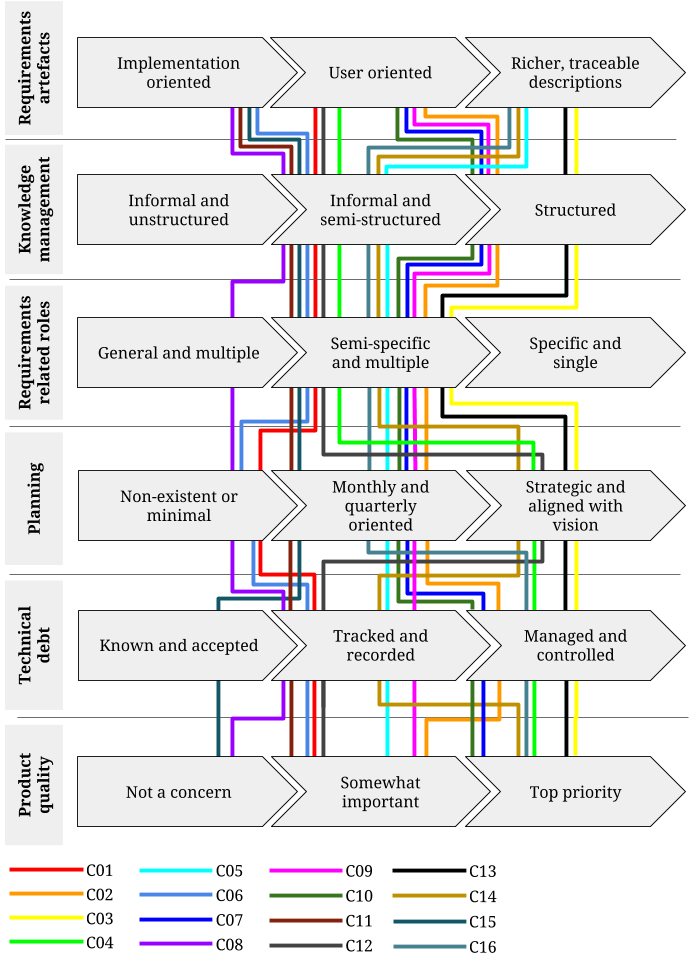
\psfig{file=companies-dimensions.png,width =3.4in}
\caption{Phases of Evolution along the Six Dimensions by Company}
\label{fig:companiesEvolution}
\end{figure}

\subsection{Research Methods}
\label{sec:researchMethods}
Data was collected by conducting interviews, all-day observations, and attending project meetings. To understand the evolution of requirements practices, two questions were asked at 16 software startups: how do requirements practices change, and what factors and turning points drive those changes?~\cite{Gralha:2018} These questions were used to learn about company growth, requirements gathering, requirements prioritization, features and knowledge management, and tools. The goal of that study was to determine which of the three phases of the six dimensions that each startup is currently at. 

Gralha et. al characterize each dimension by 3 phases of evolution. The first phase is the beginning phase, where practices are unstructured. In the second phase, practices are semi-structured. In the third and final phase, practices are formally structured~\cite{Gralha:2018}. Every advance from one phase to the next is caused by at least one of eight turning points: number of clients, input from clients, negative feedback, retention rate of clients, revenue, number of employees, number of remote workers or flexible work hours, and number of features or products.~\cite{Gralha:2018} Phases of evolution for each specific dimension will be explained below.

\subsection{Phases of Evolution}
\label{sec:reqPracticeEvolution}

\subsubsection{Requirements Artifacts}
In the first phase, startups begin with little or no user input because their product is still in the process of entering the market, making requirements artifacts \emph{implementation-oriented}. The founders' backgrounds and company culture determine what tasks need to be done. Tasks are informally documented, sometimes on sticky notes. The second phase is \emph{user-oriented}. Startups look at feedback and input from their users to develop new tasks that are commonly documented with project management tools such as Confluence and Jira.~\cite{Gralha:2018} In the final phase, ``requirements artifacts evolve into \emph{richer, traceable descriptions}."~\cite{Gralha:2018} Tasks are broken down into smaller, simpler tasks that are given effort-based estimations for time of completion. Tasks are formally prioritized, assigned to developers, and organized into products or releases.

\subsubsection{Knowledge Management}
Knowledge management is informal and unstructured in its first phase. Founders and developers rely on each other to complete tasks and manage the few features of their product. As the number of tasks, features, and employees grow, startups enter the second phase where knowledge management is informal and semi-structured. Knowledge is shared through regular team and company meetings. Online communication tools, such as Slack, are used in place of ad hoc verbal communication. When a startup grows to a size that separates employees into different departments, knowledge management is formally structured. Using tools such as Slack and GitHub, communication and project management are often intertwined.

\subsubsection{Requirements-Related Roles}
Startups begin with general and multiple requirements-related roles where ``everyone does everything."~\cite{Gralha:2018} Once a startup has clients, they move to the second phase where roles are semi-specific. Clients receive more attention and marketing staff are brought on, giving developers more room to focus on product development. In the final phase, roles are specific and single. Startups might decide to hire product managers and quality assurance specialists.

\subsubsection{Planning}
Startups do not have any planning in the first phase. Most time and resources are spent developing a working product that looks attractive to the market. Once a startup understands client needs, it moves to the second phase where planning is monthly and quarterly-oriented. Planning is based on client requests without deadlines. In the third phase, planning is strategic and aligned with vision. Companies prioritize features for a broader market and decide what is better for their clients.

\subsubsection{Technical Debt}
Technical debt is known and accepted in the earliest phase. As products become more complex, startups will track and record technical debt in the second phase. Hiring additional developers provides more resources to address some, but not all of a startup's technical debt. In the final phase, technical debt is managed and controlled. Tasks are specifically created to address this debt and prioritized with their associated features.

\subsubsection{Product Quality}
In the first phase, ``speed of release takes precedence over quality."~\cite{Gralha:2018} With minimal testing, there are higher rates of negative feedback due to defective features. To avoid negative feedback, startups move to the second phase where product quality is somewhat important. User experience and scalability become critical. Product quality eventually becomes a top priority in the last phase due to its correlation with company reputation.

\subsection{Discussion}
\label{sec:discussion}
In a fast-paced and reactive environment, startups ignore the long run in order to capture a market, acquire clients, and release products more quickly. Evolution along the six dimensions are not fundamental to success. Factors that cause startups to die can be a combination of the market of its product, human resources, culture, funding, processes, and practices.

Figure~\ref{fig:companiesEvolution} shows which phase of evolution of the six dimensions that each of the 16 companies was at at the time of the study. No startup reached the third phase of requirements-related roles and all had left the first phase of knowledge management. Company C06, a 10 year-old startup is only at phase one or two in every dimension.  It was reported that the work environment at C06 was stressful and had long hours. C03, one of the furthest along every dimension, was a 4 year-old startup with 11-20 employees. C03 has formal processes for most practices, employees understand the company's vision and feel confident going into product development, and technical debt is low.~\cite{Gralha:2018} These contrasting profiles indicate that movement along the three phases of evolution is not dependent on company age and size. 

\section{Participant Observations from a Software Startup CTO}
\label{sec:CTOstory}
Andrew J. Ko, a chief technology officer (CTO) of a software startup in Seattle, WA, kept a diary to document everyday happenings at his company over a three-year span.~\cite{Ko:2017} He archived more than 15,000 emails and 9,000 hours of direct experience. Ko's goal was to study developers' behavior and software startup evolution without observational bias by acting as a participant.~\cite{Ko:2017} With this data, he made several claims about software developers and startup evolution, most of which involved requirements practices. We will look at developers' behavior towards each requirements practice and apply the phases of evolution described in Section~\ref{sec:reqPracticeEvolution}.

\subsection{Requirements Artifacts}
The CEO, whose primary job was marketing and strategy, gathered customer feedback to create requirements artifacts for the engineering team. The CEO and CTO had talked with customers before making their startup, so requirements gathering was not \emph{implementation-oriented}. Ko's startup skipped the initial phase of requirements artifacts, which puts them in the second phase of evolution where requirements artifacts are \emph{user-oriented}. 

\subsection{Knowledge Management}
Ko's startup began in the first phase where documentation was ignored. Ko describes \emph{design rationale debt}, which occurs when no one remembers why a component behaved the way it did.~\cite{Ko:2017} To deal with this, they started documenting components upfront. For example, he recalled a time when they added a feature a year ago and ``could only vaguely remember why we thought it was so critical at the time ... removing the feature risked breaking an undocumented customer requirement."~\cite{Ko:2017} As more problems arose from lack of documentation, they started practicing it more frequently to be mindful of the long run. By the end of the study, the company transitioned to the second phase of evolution where knowledge management was informal and semi-structured.

\subsection{Requirements-Related Roles}
Ko's startup began with only two employees. Ko became the CTO because of his technology experience. His friend Jake Wobbok, whom he had met in college, was the CEO. Together, they started in the first phase of evolution where each role was responsible for doing everything. They made sales pitches, gathered funds, and collaborated with potential customers. Once they were able to release a product that collected revenue, they hired a team of software developers, a team for customer support, and account managers. Jake was able to focus more on marketing and Ko could focus more on their product's technology. So, at the time that the study was completed, they had moved on to the second phase of evolution where roles were semi-specific. 

\subsection{Planning}
When the startup began, Ko was the sole developer who worked on releasing a functional product without planning, which is the first phase of evolution. As their startup grew, an engineering team was hired. This entered them into the second phase of evolution where planning is based on customer feedback without deadlines. During planning sessions, however, developers found it unethical to accelerate feature development and product releases at the cost of low quality, low security software.~\cite{Ko:2017} Developers preferred to work on tasks that are interesting and challenging. Nobody wanted to work on straightforward, boring tasks.~\cite{Ko:2017} Ko describes \emph{planning debt}, in which developers maintain plans in their minds, handwritten notes, and partially completed tasks,~\cite{Ko:2017} making it difficult to transfer tasks between developers. Because of these issues, assigning tasks to developers was a challenge.

\subsection{Technical Debt}
Still need to write about technical debt at Ko's startup.

\subsection{Product Quality}
Still need to write about product quality at Ko's startup.

\section{Conclusions}
\label{sec:conclusions}

\section*{Acknowledgments}
\label{sec:acknowledgments}

Thanks Elena and Nic!

% The following two commands are all you need in the
% initial runs of your .tex file to
% produce the bibliography for the citations in your paper.
\bibliographystyle{abbrv}
% sample_paper.bib is the name of the BibTex file containing the
% bibliography entries. Note that you *don't* include the .bib ending here.
\bibliography{hoff_senior_sem}  
% You must have a proper ".bib" file
%  and remember to run:
% latex bibtex latex latex
% to resolve all references

\end{document}
